\documentclass[12pt,letterpaper]{exam}

\newcommand{\DocTitle}{Renew the DocTitle variable.}
\newcommand{\CourseNumber}{NE555}
\newcommand{\CourseName}{Nuclear Reactor Dynamics}
\newcommand{\DayTime}{TuTh 8:00-9:15}
\newcommand{\Room}{VV\&E B129}
\newcommand{\Term}{Spring 2011}
\newcommand{\Instructor}{Lewis John Lloyd}
\newcommand{\School}{University of Wisconsin - Madison}

\usepackage{listings}
\usepackage{mathtools}
\usepackage{xtab}
\usepackage{longtable}
\usepackage{array}
\usepackage{mathrsfs}
\usepackage{color}
\usepackage{multicol}
\usepackage{pdflscape}
\usepackage{pdfpages}
\usepackage{graphicx}
\usepackage{esint}
\usepackage{amsmath}
\usepackage{amssymb}
\usepackage{graphics}

\usepackage[
			pdfborder={0 0 0},
			urlcolor=cyan,
			pdftitle={\CourseNumber \DocTitle},
			pdfauthor={\Instructor}
			]{hyperref}
			
\usepackage[
			includeheadfoot,
			top=0.5in,
			bottom=0.5in,
			left=1.0in,
			right=1.0in
			]{geometry}
\setlength{\parindent}{0in}
\setlength{\parskip}{\baselineskip}

\lhead{\CourseNumber: \CourseName}
\chead{}
\rhead{\Term}
\lfoot{}
\cfoot{\thepage}
\rfoot{}
\coverlhead{\CourseNumber: \CourseName}
\coverchead{}
\coverrhead{\Term}
\coverlfoot{}
\covercfoot{\School}
\coverrfoot{}


\correctchoiceemphasis{\bfseries\color{red}}
\bracketedpoints
\pointsinmargin
%\addpoints
%\shadedsolutions

\lstset{ %
language=Matlab,                % the language of the code
basicstyle=\footnotesize,       % the size of the fonts that are used for the code
numbers=left,                   % where to put the line-numbers
numberstyle=\footnotesize,      % the size of the fonts that are used for the line-numbers
stepnumber=5,                   % the step between two line-numbers. If it's 1, each line 
                                % will be numbered
numbersep=5pt,                  % how far the line-numbers are from the code
backgroundcolor=\color{white},  % choose the background color. You must add \usepackage{color}
showspaces=false,               % show spaces adding particular underscores
showstringspaces=false,         % underline spaces within strings
showtabs=false,                 % show tabs within strings adding particular underscores
frame=single,                   % adds a frame around the code
tabsize=2,                      % sets default tabsize to 2 spaces
}

\renewcommand{\solutiontitle}{\noindent\textbf{Solution:}\par\noindent}

\newcommand{\mathsym}[1]{{}}
\newcommand{\unicode}{{}}
\newcommand{\tr}[1]{\tilde{#1}}
\newcommand{\LapTran}[1]{\mathscr{L}\left[#1\right]}
\newcommand{\InvLapTran}[1]{\mathscr{L}^{-1}\left[#1\right]}
\newcommand{\ParDer}[2]{\frac{\partial #1}{\partial #2}}
\newcommand{\Der}[2]{\frac{d\; #1}{d\;#2}}


\renewcommand{\DocTitle}{Problem Set 04}
\noprintanswers

%-------------------------------------------------------------------------------------
\begin{document}
%-------------------------------------------------------------------------------------
\begin{center}
\textbf{\DocTitle}
\end{center}
%-------------------------------------------------------------------------------------
\begin{questions}
%-------------------------------------------------------------------------------------
\question{
	This problem deals with the following differential equation:
 $$\displaystyle \frac{d u(t)}{d t} = \lambda\left(u(t)-cos(t)\right)-sin(t),\; u(t_o) = \eta$$
The analytical solution to this differential equation given by:
 $$\displaystyle u(t) = e^{\lambda\;(t-t_o)}(\eta-cos(t_o))+cos(t)$$	

	\begin{parts}
		\part[10]{
		Let $\lambda$, $t_o$, and $\eta$ be $-2100$, $0$ and $1.0$, respectively.
		What is the maximum time step possible to achieve a stable algorithm for Forward Euler?
		Answer the question analytically following the procedure presented in class.
		}
		\part{
		Let $\lambda = -10^{6}$, $t_o = 0$ and $\eta = 1.0$ be the data for the following subparts.
			\begin{subparts}
				\subpart[10]{
				Use the Backward Euler method to numerically solve the differential equation out to $t=4.0\;[s]$.
				Use the following five time step sizes: $k = (0.5,0.1,0.05,0.01,0.005)$.
				Report the difference between the numerical solution and the analytic, $abs\left|U^{N}-u\right|$, solution at $t=4.0\;[s]$ for each time step size.
					\fullwidth{
						\begin{solution}
					
						\end{solution}
					}
				}
				\subpart[10]{
				Use the Trapezoidal method to numerically solve the differential equation out to $t=4.0\;[s]$ with the following five time step sizes: $k = (0.5,0.1,0.05,0.01,0.005)$. Report the difference between the numerical solution and the analytic, $abs\left|U^{N}-u\right|$, solution at $t=4.0\;[s]$ for each time step size.
					\fullwidth{
						\begin{solution}

						\end{solution}
					}
				}
			\end{subparts}
		}
		\part{
		Let $\lambda = -10^{6}$, $t_o = 0$ and $\eta = 1.5$ be the data for the following subparts.
			\begin{subparts}
				\subpart[10]{
				Use the Backward Euler method to numerically solve the differential equation out to $t=4.0\;[s]$ with the following five time step sizes: $k = (0.5,0.1,0.05,0.01,0.005)$. Report the difference between the numerical solution and the analytic, $abs\left|U^{N}-u\right|$, solution at $t=4.0\;[s]$ for each time step size.			
					\fullwidth{
						\begin{solution}

						\end{solution}
					}
				}			
				\subpart[10]{
				Use the Trapezoidal method to numerically solve the differential equation out to $t=4.0\;[s]$ with the following five time step sizes: $k = (0.5,0.1,0.05,0.01,0.005)$. Report the difference between the numerical solution and the analytic, $abs\left|U^{N}-u\right|$, solution at $t=4.0\;[s]$ for each time step size.		
					\fullwidth{
						\begin{solution}

						\end{solution}
					}
				}
			\end{subparts}
		
		}
	\end{parts}
}
%-------------------------------------------------------------------------------------
\end{questions}

\ifprintanswers
\begin{landscape}
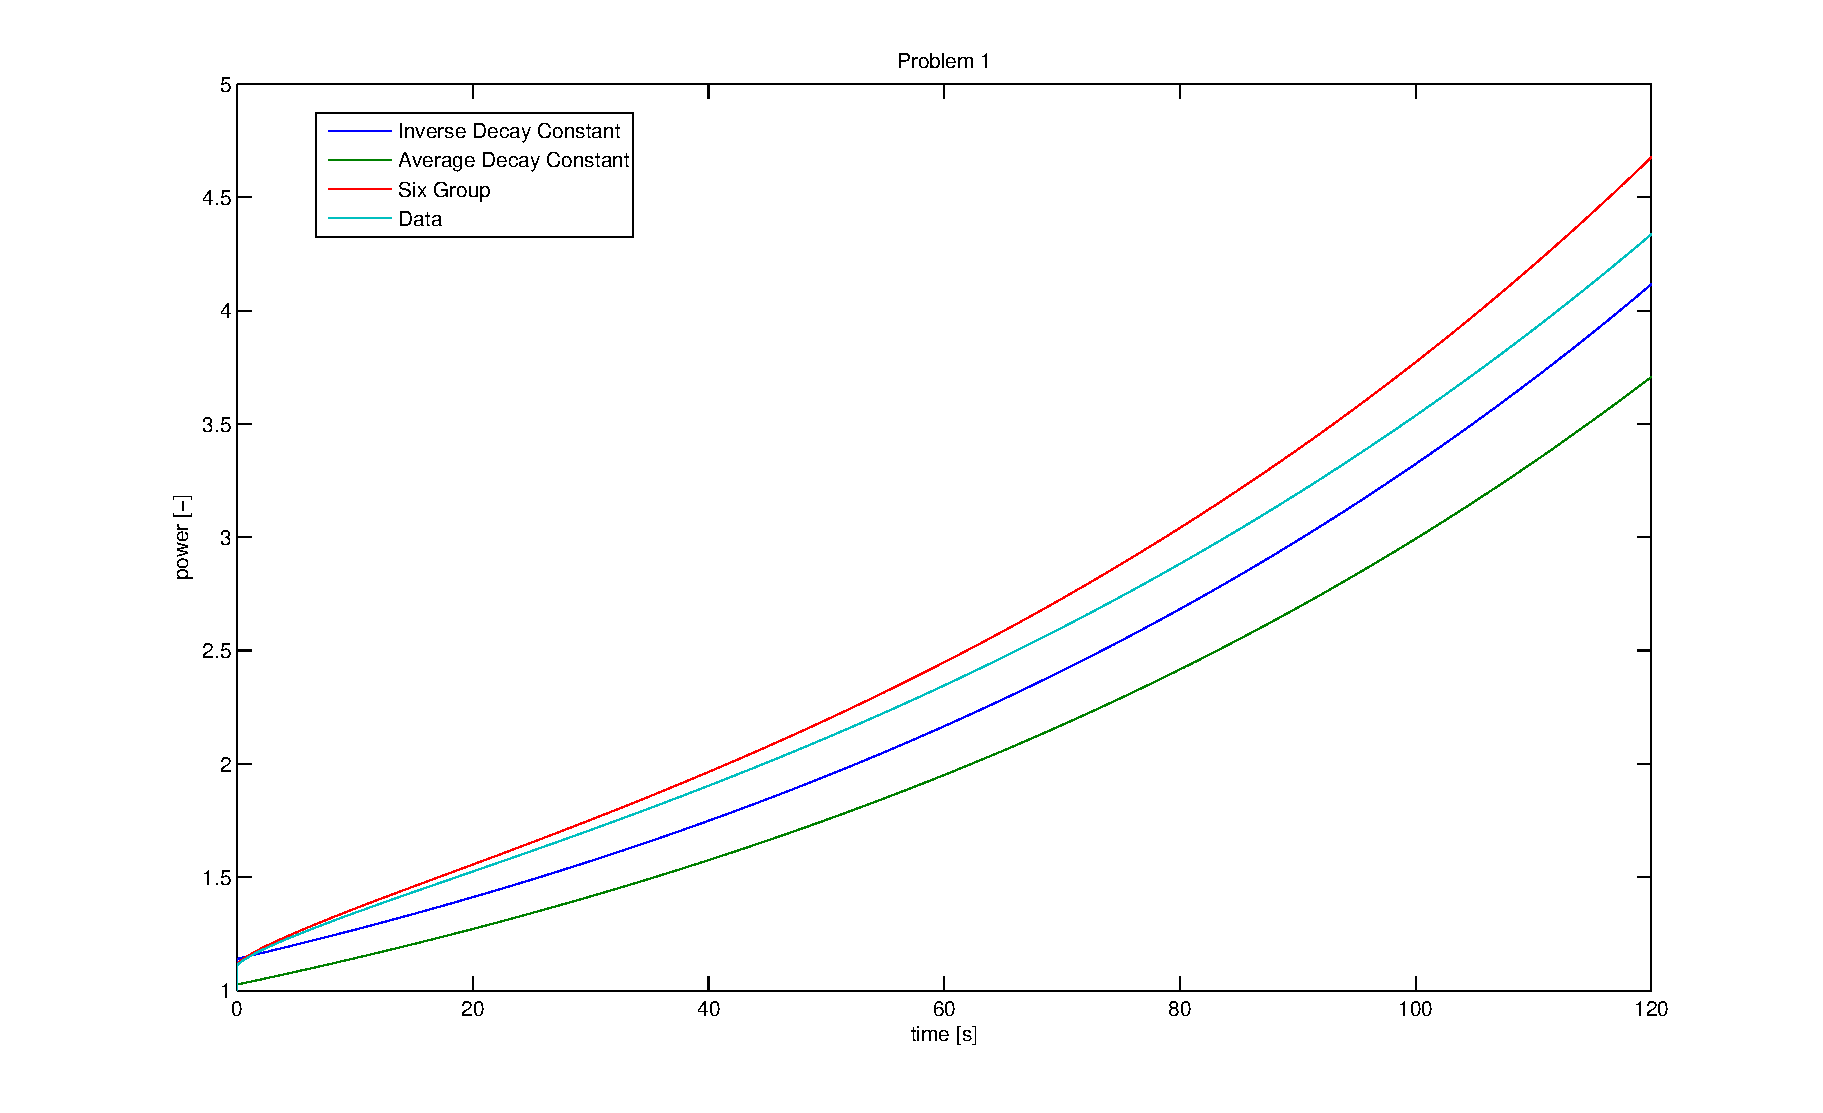
\includepdf[landscape=true]{PS03Q01pic.pdf}
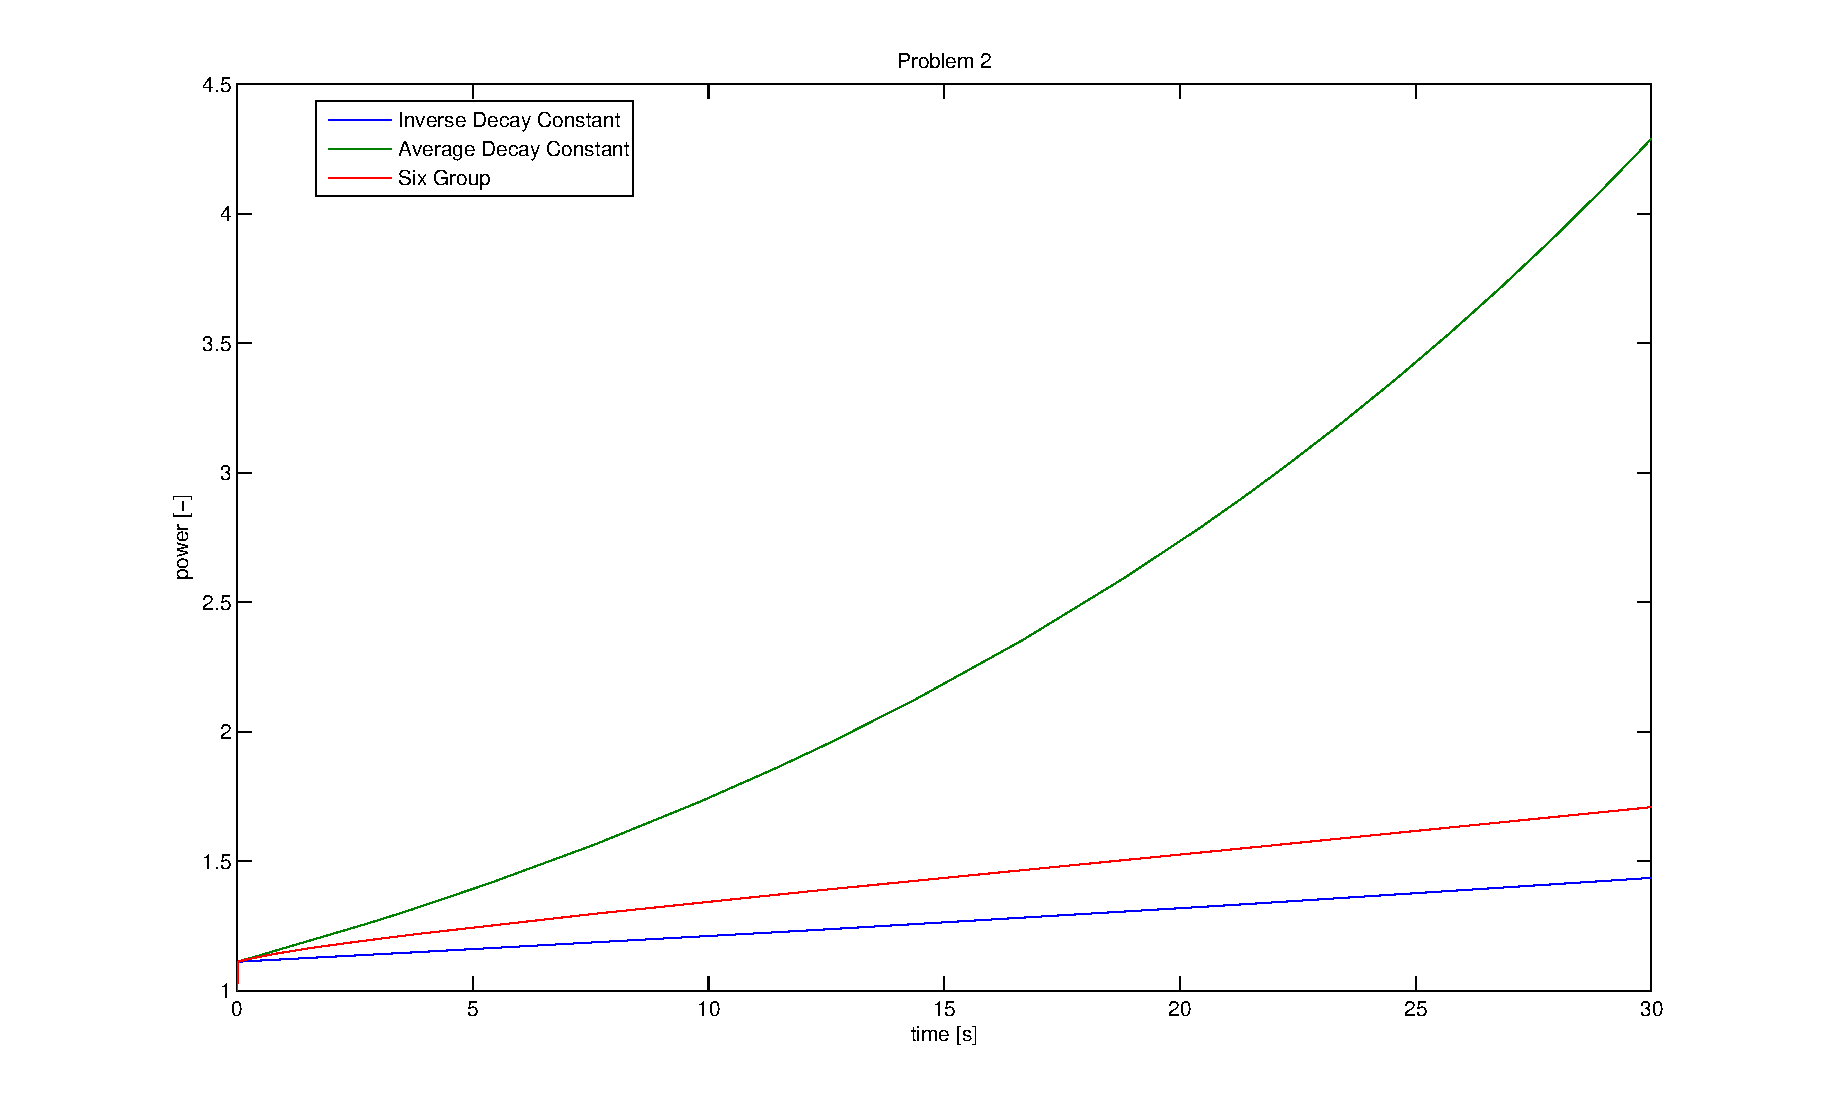
\includepdf[landscape=true]{PS03Q02pic.pdf}
\end{landscape}
\fi

\end{document}